\documentclass[12pt, twoside,a4paper]{report}
\oddsidemargin = 10pt
\textwidth = 430pt

\usepackage{fullpage}	 %to make smaller margins
\usepackage{graphicx}
%\usepackage[utf8]{inputenc}
%\usepackage[T1]{fontenc}
%\usepackage{url}
\usepackage{hyperref}
\usepackage{pdfpages}
%\usepackage{placeins}
\usepackage{graphicx}
\usepackage{caption}

\usepackage{epstopdf}
\usepackage{subcaption}
\usepackage{enumerate}
\usepackage{amsmath}
\usepackage{listings} %for showing program code

\lstset{backgroundcolor={\color{white}}, %old formatting for program listings I used in my bachelor thesis ;)
basicstyle={\bfseries\ttfamily\footnotesize},
breakatwhitespace=false,
breaklines=true,
captionpos=b,
columns=fullflexible,
commentstyle={\color[rgb]{0.133,0.545,0.133}},
escapeinside={\%*}{*)},
fontadjust=true,
frame=single,
identifierstyle={\ttfamily},
keywordstyle={\bfseries\ttfamily\color[rgb]{0,0,1}},
language=C++,
numbers=left,
numbersep=5pt,
numberstyle={\footnotesize},
showspaces=false,
showstringspaces=false,
showtabs=false,
stepnumber=1,
stringstyle={\ttfamily\color[rgb]{0.627,0.126,0.941}},
 morekeywords={vec2,vec3,vec4,mat2,mat3,mat4,in,uniform,version,out},
tabsize=2}

\usepackage{wrapfig}
\usepackage{lipsum}
\usepackage{float}
\usepackage{titlesec}	

\titlespacing*{\section}{0pt}{0pt}{20pt}

\setlength{\intextsep}{0pt} %to make wrapfigures beautiful
\setlength{\oddsidemargin}{0.5cm}
\setlength{\evensidemargin}{-0.5cm}
\begin{document}


\begin{titlepage} \vspace*{-20mm}
 %
\begin{minipage}[b]{20mm}%
\includegraphics[height=10mm]{front/DTU_Informatics_logo}\\[-1.5mm] %
\end{minipage}\hfill{}\includegraphics[height=15mm]{front/DTULogo} \\[10mm]

\centering \parindent=0pt \global\long\def\HRule{\rule{\textwidth}{1mm}}


\textsc{High-Performance Computing, }02614\\


\vspace*{\stretch{1}} \HRule\\[.5cm]\textbf{\textsc{\Huge Assignment 1: Matrix Multiplication}}{\Huge \par}


\textbf{\Huge \HRule\\[1cm] \includegraphics{front/DTULogo}}{\Huge \par}

\textbf{\Huge \\[2cm] }{\Huge \par}
\textbf{\Large GROUP:\\[1cm] }{\Huge \par}
\textsc{\large Alessandro Dal Corso  (s120929)}{\large }\\
{\large{} }\textsc{\large Alexander Birke  (s124044)}{\large }\\
{\large{} }\textsc{\large Daniele Brazzolotto  (s111071)}{\large }\\
{\large{} }{\large \par}

\textsc{\large \vspace*{\stretch{2}} }{\large \par}

\begin{flushleft}
\textsc{Technical University of Denmark}\\
 \textsc{ %{\large \today}
Lyngby, $15^{\mathrm{th}}$ January 2013 } 
\par\end{flushleft}

\end{titlepage} 



\tableofcontents
\clearpage
\chapter{Assignment 1}

\section{Summary}
The ultimate goal of the assignment is implementing a matrix multiplication algorithm, optimized for single CPU, single core machine. The focus is on how an existing code can be speeded up, without changing (too much) the total number of operations.

An iterative process has been used to improve the code and, after every optimization, an automatic test session has been performed in order to verify the actual performances on different conditions. In some interesting case a profiling tool has been used to investigate in depth some specific behaviour.

The results confirmed that the main bottleneck of the naive algorithm was the poor use of the cache, but they also saw that the best performances can be reach with code that leads to the right compiler optimizations, rather than with code that pretends to optimize everything itself. 


\section{Problem Statement}
From the assignment we were given the following tasks

\begin{itemize}
\item Write a function that performs matrix matrix multiplication on arbitrary sized two-dimensional arrays.
\item Make a separate implementation for each way the loops in the above function can be ordered and test which one is the fastest.
\item Compare the result of our implementation to DGEMM(), a similar function in the BLAS library
\item All the functions and the call to DGEMM() should be wrapped into a single library.
\item Implement a blocked version of the matrix matrix multiplication function and identify the block size that gives the best performance in regards to L1 cache. This result should be compared to the timings for the library function.
\item Compare different compiler settings to see how they affect the result.

\end{itemize} 

\section{Description of Hardware and Software Used}
 - stuff from lscpu
 - compiler and libraries used. version numbers to
 


\section{Theory}
The matrix multiplication is a critical operation in computer science, both because it is the base of several practical problems and because it is still relatively expensive. \\
This operation, in fact, is really the fundamental brick of several interesting problems, from the resolution of big linear systems, often applied to physics, to resolution of discrete Fourier transforms, used for example to DNA splicing problems.
On the main challenges of this operation is not related to the pure computational power, but with the amount of data that it requires: nowadays, as CPU/GPU evolved and still evolves faster than the memory chips, the real challenge is not to compute the result in a short time, but making the computational unit able to produce that result. In other words, it is more expensive bringing the right data at the right time, to the right chip, than to actually produce the result. \\
Algorithms in general nowadays, are so much affected by this behaviour, that the fastest ones are the algorithms that make a better usage of the caches.
From this point of view, matrix multiplication is considered a good example of what a typical algorithm should look like these days. It is therefore used as a base to test the ability of high performances computers to deliver outcomes. 
\\\\
\section{Loop Optimization Techniques}
Since scientific computing often requires the looping over large data sets there has been developed multiple optimization strategies that targets different areas. These areas are:
\\\\
\textbf{Spatial locality}\\
Reuse all the data fetched in a single cache line. Optimization techniques that leads to this is blocking.
\\\\
\textbf{Temporal locality}
Reuse data in previously fetched cache lines. Optimization techniques that leads to this is blocking.
\\\\
\textbf{loop bookkeeping}\\ 
This is the overhead of running the loop in the first place. This happens when the loop only does a small amount of computation. Techniques that addresses this are loop unrolling and loop fussion. 
\\\\
\textbf{Vectorization}\\
Modern CPU's contain units that can do floating point operations on more than one value at a time. If a loop is organised in a proper way and if the results calculated in the loop is not dependent upon each other it can be recognized by the compiler and assembler code will be generated that takes advantage of these units. Loop fission can help the compiler to do this. 
\\\\
Since loop blocking will be used later in this report we will cover it in more detail here.
\section{Loop Blocking}
A common technique to improve temporal and spatial locality at the cost of loop overhead is blocking. This technique takes a multi dimensional array and splits the computation on it up into smaller blocks. The size of the block is chosen to fit inside the cache size. This ensures that the cache is only filled with data that will be used in the current computations and later implementations. Blocking is implemented by having a set of loops that iterates over the blocks and then have a second set of loops inside the first set that iterates over each element. An implementation of this that calculates the transpose of matrix in C is shown below: 
\begin{lstlisting}
for(int i = 0 ; i < n ; n += nbi)
	for( int j = 0 ; j < n ; j++)
		for( int k = 0 ; k < min(n-i, nbi) ; k++)
			A[j][i+k] = B[i+k][j]
\end{lstlisting}
The above loop accesses array A in a column wise order which in C usually results in many cache misses but because this is only done for as much memory as there can be in the cache it means that the data that has been fetched once in one cache page can be used again in a later iteration of the loop.
\\\\
Blocking is a powerful technique to improve memory use and data reuse but also has its disadvantages. The optimal block size is dependent on the CPU the code is being run on and on what data the algorithm is used on. It is therefore a good idea to have parameters to specify the block size so the implementation can be ported to different architectures more easily.

\section{Implementation}
- write something about test scripts



\section{Results and Conclusions}
 
\section{Comparison against dgemm}

Against the dgemm library function, even with the same compiling options, the implementation provided of the matmult\_nat() method has been proven poor, according to the graph shown in Figure \ref{fig:natdgemmcomp}. The figure shown that, for every possible permutation of the cycle order (including so the naive implementation), dgemm outnumbers it.

\begin{figure}[here]
\centering
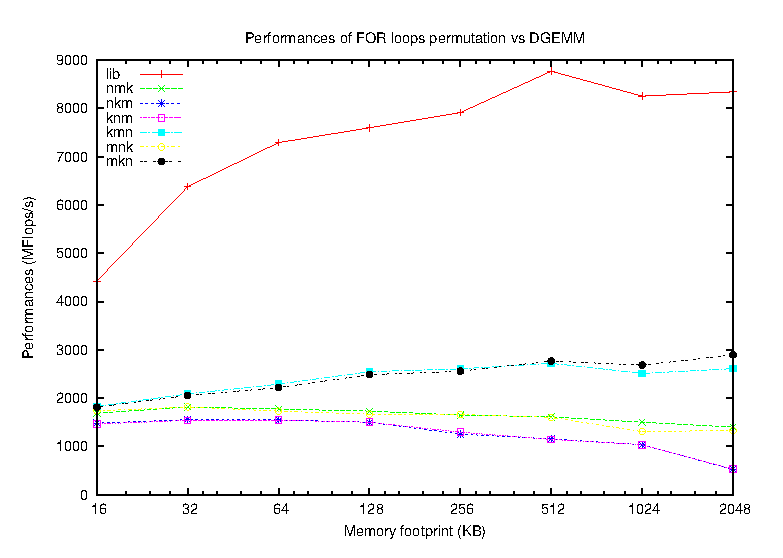
\includegraphics[width=\textwidth]{results/dgemm.eps}
\caption{Comparison between \emph{dgemm()} and the other implementations.}
\label{fig:natdgemmcomp}
\end{figure}


The reason for that ... (investigation required)

\section{Permutations of m, k, n and performance}
The three cycles performed in the naive algorithm can be rearrenged in six different ways: there are in fact six possible permutations of the three letters. The performance results provided by the execution of the six algorithms on some standards memory footprints are provided in Figure \ref{fig:permutations}. The test was made on the product of square matrices $nxnxn$, where $n$ was calculated using the following formula, to relate it to the memory footprint:

\begin{figure}[here]
\centering
\includegraphics[width=\textwidth]{results/permutations.eps}
\caption{The possible combinations of \emph{matmult\_xxx()} for the Intel processor on square matrices of growing size.}
\label{fig:permutations}
\end{figure}


$$
n = \sqrt{\frac{F_{byte}}{8 \cdot 3} }
$$

The best results of the graph are the ones where the most internal cycle is cycled over $[1,n]$, and in particular the best implementation has been proved $m-k-n$, followed by $k-m-n$. The worst ones, instead, have been proved $n-k-m$ and $k-n-m$, the ones with the most internal cycle in m.

The result was what we expected in the Theory section. As a recall, the explanation of this behaviour is that $m-k-n$ is the best implementation because is the one that causes the less cache misses. If the most internal variable looped is $n$, in fact, we read a whole row in the matrix each time we start reading an element from matrices $B$ and $C$ (that have both $n$ columns). This causes less misses in the cache, leading to a better perfomance for both the $m-k-n$ and $k-m-n$ behaviours. In addition, since the A matrix has k columns, also if we loop through k before looping though m we got a better performance, for the same reason. This explains why $m-k-n$ is slighly better that  the $k-m-n$ implementation.

The worst case scenarios  $n-k-m$ and $k-n-m$, instead, do the opposite: they privilegiate columns over rows, resulting in a better performance if the matrix was stored column-wise, like in Fortran, but leading to disastruous results in C, where the most performant is the rowmajor order.

To verificate our assumption, we checked the number of cache misses for both the best and the worst implementation, resulting in the following table:

That confirmed our assumptions, seeing that the best implementation has fewer cache misses that the worst one.

\section{Performance of n,k,m implementations with different sizes}
The results and conclusions presented in the previous section held keeping in mind that the matrices we tested were square ones, where $n=m=k$. We repeated the same tests for some odd-sized matrices, i.e. where one of the three dimensions $n$,$m$,$k$ was kept at a low value (in these tests 4 elements). The other two values were raised accordingly, in order to maintain the same memory footprint and have meaningful results. The results we came up for n and am were pretty much the same, but we k we found some different results, which are presented on Figure \ref{fig:lowk}.

\begin{figure}[here]
\centering
\includegraphics[width=\textwidth]{results/littlek.eps}
\caption{The possible combinations of \emph{matmult\_xxx()} with AMD processor.}
\label{fig:lowk}
\end{figure}

We can see that the performances of the two best version in the square case are dropped dramatically, especially for little memory footprints. Since the test is on the AMD processor, we are able do see a drop in the performance due to the filling up of the L1 cache around $128kB$ (the cache is actually 64K, but it seems a little larger due to prefetch). For matrix sizes, we can see that the results of the cache analysis still confirm our previous assumptions of $m-k-n$ being faster than $knm$, as shown in the following table:

\section{Blocked Matrix performance}
We recall that the blocked version, introduced in section //TODO, uses the best algorithm for naive multiplication, mkn, in its inner loop. We experimented the block size against the MFLOPs generated for a generally big square matrix (with 2048kB memory footprint). The results are reported in Figure //TODO (green line). The performances of the algorithm increased at the rising of the block size. This means that the optimum is the highes possible value of the block size, i.e. the matrix itself. In conclusion, the blocking algorithm is useless, because it will be always beaten by the nkm algorithm. 

\begin{figure}[here]
\centering
\includegraphics[width=\textwidth]{results/blkwrong.eps}
\caption{The possible combinations of \emph{matmult\_xxx()} with AMD processor.}
\label{fig:lowk}
\end{figure}

To find an approximate optimum for the block size, it was necessary to substitute the algorithm in the inner loop with the worst one (knm). Repeating the test, the data showed a plateau curve, having its maximum in the range 27-37. After 40, the performances start to decrease, because the L1d cache starts to fill up. At 40, in fact, we have an estimated data cache size of $3 \cdot 40^2 \cdot 8 = 37.5kB$, which is sligthly higher than the l1d cache size ($32kB$) due to the prefetching effect.  

\begin{figure}[here]
\centering
\includegraphics[width=\textwidth]{results/3way.eps}
\caption{Comarison between $dgemm()$, the best blocked version and the $m-k-n$ Implementation.}
\label{fig:3way}
\end{figure}

\section{Compiler parameters}

//TODO Alexander




%\appendix
\end{document}